
This chapter presents the methodological framework used to evaluate BPCRR for binary dispersal traits. The aim is to assess how BPCRR performs in a binary-trait setting, and to investigate whether a Gaussian linear approximation is sufficient for prediction of binary traits and estimation of breeding values. The chapter begins by describing the empirical data from the Helgeland house sparrow system, including the response variables, genomic and environmental data, and the data subsets used in the analyses. The general statistical model formulations used throughout the thesis are then introduced, contrasting a binomial model for binary responses with a linear model fitted on the observed $0/1$ scale. Following this, a simulation study is presented in which binary phenotypes are generated under a known marker-based genetic architecture, making it possible to evaluate predictive performance and recovery of the underlying genetic signal. The chapter concludes by describing the empirical analyses of dispersal, including selection of the number of principal components, comparison between BPCRR and genomic animal models, and cross-validation of estimated breeding values for downstream analyses.

\section{Data Description}

The data motivating this project come from a long-term study of a meta-population of house sparrows on an island system off the coast of Helgeland in northern Norway. The meta-population spans 18 islands divided into two main habitat types: the \textit{inner islands}, situated closer to the mainland, and the \textit{outer islands}, further from the mainland. Extensive fieldwork conducted during breeding seasons and autumns since $1993$ has ensured that most individuals have been marked and followed from hatching to death, with blood samples collected for DNA extraction and genotyping (\cite{saatoglu_genetic_2024}). Although some islands are more isolated than others, there is gene flow between all of them through dispersal (\cite{ranke_spatial_2021}), as illustrated in Figure~\ref{fig:dispersal on the map}. The resulting dataset combines genomic data with phenotypic and environmental observations, enabling the prediction of individual dispersal phenotypes and the estimation of their heritable component.

% image of map fo area
\begin{figure}
    \centering
    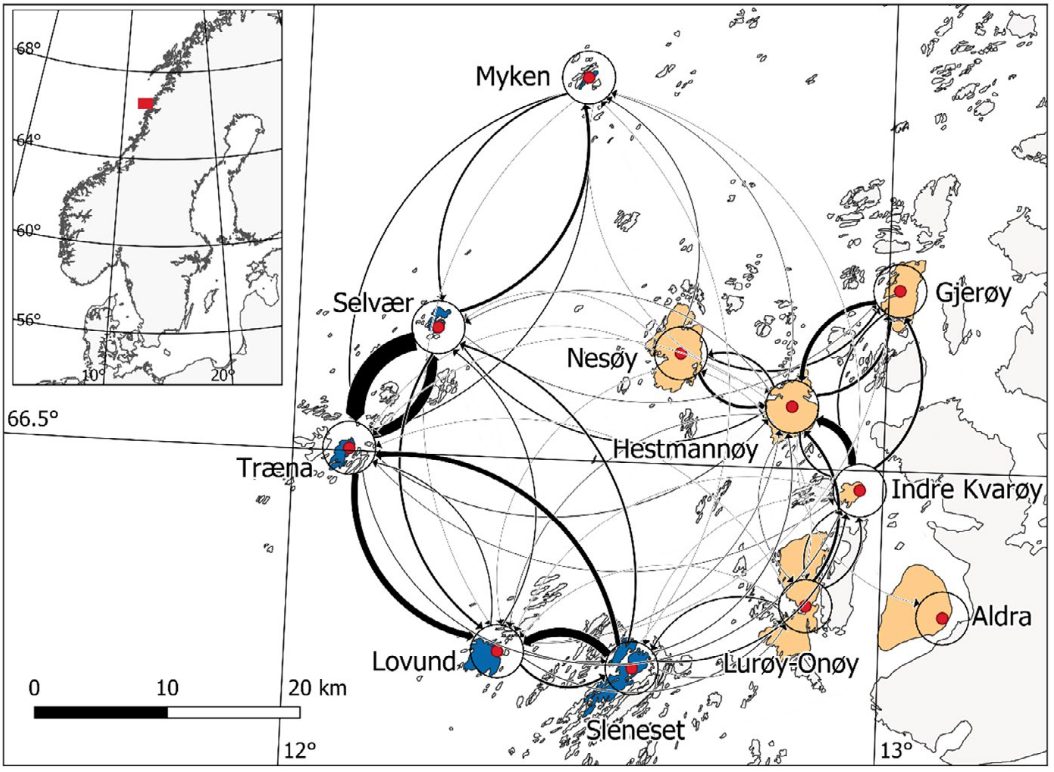
\includegraphics[width=0.8\linewidth]{Figures/Methods/Dispersal (ranke).png}
    \caption[Map of study area]{Map of the study area. Inner islands are in yellow, and outer islands are in blue. The arrows display emigration patterns in the period $1993-2014$. Increased thickness of the arrows indicates a larger volume of emigration (\cite{ranke_spatial_2021}).}
    \label{fig:dispersal on the map}
\end{figure}


\subsection{Response Variables}

The primary response variable is natal dispersal, defined as whether an individual recruited on a different island than the one it hatched on. This is recorded as a binary phenotype ($y = 1$ for dispersers, $y = 0$ for non-dispersers) at the point of recruitment. Breeding dispersal, moving between breeding seasons after first recruitment, is negligible in this system, occurring in fewer than $0.02\%$ of individuals (\cite{saatoglu_genetic_2024}), meaning that the dispersal phenotype effectively captures a single, discrete life-history decision. This trait is the focus of the main analyses: model comparison between binary and Gaussian BPCRR formulations, and estimation of individual breeding values for dispersal.

The secondary response variable is autumn dispersal, which captures whether an individual had already moved from its natal island by the time of autumn observations, prior to recruitment. This is a biologically distinct phenomenon from natal dispersal: it is observed at the nestling stage, before the individual has survived to recruit, and therefore captures early-life dispersal events that are invisible to the primary phenotype, since having a recorded dispersal phenotype includes survival through the first year (recruitment). Critically, individuals that disperse in autumn but die before recruiting are assigned $y = 1$ for autumn dispersal but receive no dispersal phenotype in the main dataset. This trait was not used for model comparison, but was included in analyses evaluating the robustness of the estimated breeding values.

\subsection{Genomic and Environmental Data}

For each individual, a blood sample was collected for DNA extraction and genotyping, yielding $M = 65\,244$ SNPs per individual. In addition to the genomic data, a set of environmental covariates was recorded for each individual, as listed in \autoref{tab:environmental covariates}. The dataset spans yearly observations from $1993$ to $2019$, and contains $N = 4722$ unique individuals with a recorded dispersal phenotype, of which $1106$ ($23\%$) dispersed. An additional $4306$ individuals did not recruit and therefore have no dispersal phenotype, but are retained in the dataset for the down stream analysis. For the autumn dispersal trait, the phenotype was recorded for a subset of $1142$ nestlings from $2007$--$2014$ for which both nest observations and autumn observations were available in the same year. Among these, $105$ ($9\%$) had dispersed by autumn, of 
whom $50$ did not subsequently recruit.

%table of environmental components
\begin{table}[h!]
\centering
\caption{Environmental features included in the dataset.}
\vspace{6pt}
\label{tab:environmental covariates}
\begin{tabular}{ll}
\hline
\textbf{Feature} & \textbf{Description} \\
\hline
Ringnr        & Unique individual identifier \\
HatchYear     & Year the individual hatched \\
Natal Island  & Island where the individual hatched \\
Adult Island  & Island of recruitment  \\
Sex           & Sex of the individual  \\
Recruit       & Survival to recruitment \\
$\text{F}_\text{ROH}$  & Inbreeding coefficient \\
\hline
\end{tabular}
\end{table}

%It should be noted that $115$ individuals in the dataset originated from Vega, an island outside the core study area. Because Vega is not part of the monitored meta-population, only individuals that dispersed from Vega into the Helgeland system 
are present in the dataset. This means the Vega subsample consists exclusively of dispersers ($y = 1$), and is therefore not a representative sample of the Vega population. 
%The implications of this for the analyses are described in 
%Section~\ref{sec:data_subsets}.


\subsection{Data Subsets}
\label{sec:data_subsets}

Before fitting the empirical models, the dataset was examined to identify individuals 
whose dispersal status was not directly comparable to the within-system dispersal 
phenotype. A total of $115$ individuals originated from Vega, an island outside the 
core study area, and as described in Section~\ref{sec:genomic_data}, this subsample 
consists exclusively of dispersers and is not representative of the Vega population. 
To avoid this bias influencing model evaluation, these individuals were excluded from 
the reduced dataset used in the main analyses. This exclusion was applied to the 
comparison of the binomial and Gaussian BPCRR models, the comparison with the 
Bayesian animal model, and the ranking-based model comparisons.

For analyses where the goal was not model evaluation but rather the generation of 
breeding value predictions for all available individuals, the excluded individuals 
were re-included. This full dataset was used solely for the downstream prediction of 
breeding values, which form the basis for analyses conducted outside the scope of 
this thesis.

%The autumn dispersal dataset, was used exclusively as a tool for evaluating the robustness of the breeding values estimated from the primary dispersal trait. Specifically, it was used to assess whether breeding values estimated from natal dispersal are predictive of autumn dispersal status, contributing to a broader investigation of the relationship between dispersal breeding values and fitness-related outcomes.



\section{Statistical Models}\label{sec:stat_mod}

In this section, we define the general statistical models used throughout the thesis. 
The analyses compared a binary model formulation with a linear model formulation.
For $N$ individuals, the binomial model was defined through the linear predictor
%
\begin{equation}
\label{eq:method_bin_lin_pred}
\boldsymbol{\eta}
=
\beta_0 \mathbf{1}_N
+
\mathbf{X}\boldsymbol{\beta}
+
\mathbf{W}\mathbf{d}_0
+
\mathbf{a} \ ,
\end{equation}
%
%\eqref{eq:method_bin_lin_pred} and~\eqref{eq:bin_prob}.
where $\boldsymbol{\eta}$ was the $N \times 1$ vector of linear predictors, 
$\beta_0$ was the intercept, and $\mathbf{1}_N$ is an $N \times 1$ vector of ones. 
The matrix $\mathbf{X}$ was an $N \times P$ design matrix for the fixed effects, 
with corresponding coefficient vector $\boldsymbol{\beta} = (\beta_1,\ldots,\beta_P)^\top$. 
Similarly, $\mathbf{W}$ was an $N \times J$ design matrix for the random effects, 
with corresponding vector of random-effect coefficients 
$\mathbf{d}_0 = (d_{0,1},\ldots,d_{0,J})^\top$. 
The breeding values were also included as a random effect, and were assumed to follow
%
\(
\mathbf{a} \sim N(\mathbf{0}, \Sigma_{\mathbf{a}}) \ ,
\)
%
for some additive genetic covariance structure $\Sigma_{\mathbf{a}}$.

For the binomial model, the expected response was obtained by applying the inverse logit link function to the estimated linear predictor:
%
\begin{equation}
\label{eq:bin_prob}
\hat{\mathbf{p}}
=
\operatorname{logit}^{-1}(\hat{\boldsymbol{\eta}})
=
\frac{\exp(\hat{\boldsymbol{\eta}})}
{1 + \exp(\hat{\boldsymbol{\eta}})} \ ,
\end{equation}
%
where the transformation was applied element-wise, and $\hat{\mathbf{p}}$ denoted the vector of individual probabilities of success for the binary response.

The corresponding linear model was given by
%
\begin{equation}
\label{eq:method_gauss_mod_matrix}
\mathbf{y}
=
\beta_0 \mathbf{1}_N
+
\mathbf{X}\boldsymbol{\beta}
+
\mathbf{W}\mathbf{d}_0
+
\mathbf{a}
+
\boldsymbol{\varepsilon} \ ,
\end{equation}
%
where $\mathbf{y}$ was the $N \times 1$ response vector and $\boldsymbol{\varepsilon}\sim N(\mathbf{0}, \sigma^2_\varepsilon \mathbf{I}) $ was the error term.  
%
The expected response was given by
%
\begin{equation}
\label{eq:method_gauss_est_matrix}
\hat{\mathbf{y}}
=
\hat{\boldsymbol{\eta}}
=
\hat{\beta}_0 \mathbf{1}_N
+
\mathbf{X}\hat{\boldsymbol{\beta}}
+
\mathbf{W}\hat{\mathbf{d}}_0
+
\hat{\mathbf{a}} \ ,
\end{equation}
%
where a hat, $\hat{\cdot}$, denoted the estimate of the corresponding model component. 
Specifically, $\hat{\mathbf{y}}$ was referred to as the predicted linear dispersal score.

Throughout the thesis, all models are fitted within a Bayesian framework using INLA 
(\cite{rue_approximate_2009}). Penalized complexity priors are assigned to the random-effect components, and the random effects are estimated from their posterior distributions. As the breeding values are modelled as random effects, the estimated breeding values are taken to be the posterior means of their corresponding marginal posterior distributions.  


\section{Representations of the Additive Genetic Component}

The models introduced above include an additive genetic component, $\mathbf{a}$, which captured genetic contributions to individual variation in the response. In the analyses presented in this thesis, this component was represented in two different ways. First, we used a marker-based Bayesian Principal Component Ridge Regression (BPCRR) approach, where genetic effects were expressed through principal components derived from the SNP matrix. Second, we used a Bayesian genomic animal model, where marker information was incorporated through the covariance structure of the breeding values via a genomic relationship matrix (GRM).

\subsection{Bayesian Principal Component Ridge Regression Representation}

In the BPCRR models, the additive genetic component was represented using the first $K$ principal components of the SNP matrix. Following the framework of \textcite{aspheim_flexible_2026}, the breeding values are approximated as a linear combination of marker-derived principal components,
%
\begin{equation}
\mathbf{a}_K^\star = \mathbf{Z}_K^\star \boldsymbol{u}_K^\star ,
\label{eq:PC_representation}
\end{equation}
%
where $\mathbf{Z}_K^\star$ contains the first $K$ principal components and $\boldsymbol{u}_K^\star$ denotes the corresponding vector of PC effects. 

\subsubsection*{Scaling the PCs}
Before fitting the BPCRR models, the PCs were scaled following the approach of 
\textcite{aspheim_flexible_2026}. In standard ridge regression, predictors are often standardized to have equal variance (\cite{gianola_priors_2013, aspheim_flexible_2026}). For PCs derived from SNP data, however, we wanted to retain the relative amount of marker variation captured by each component. The PCs were therefore scaled such that their variances remained proportional to the corresponding eigenvalues of the SNP matrix, while being bounded for numerical stability. Let $\tilde{\mathbf{Z}}_k$ denote the $k$th unscaled PC. The scaled PC was defined as
%
\[
\mathbf{Z}_k^\star =
\frac{\tilde{\mathbf{Z}}_k}
{\sqrt{\mathrm{Var}(\tilde{\mathbf{Z}}_1)}} ,
\]
%
so that
%
\[
\mathrm{Var}(\mathbf{Z}_k^\star)
=
\frac{\mathrm{Var}(\tilde{\mathbf{Z}}_k)}
{\mathrm{Var}(\tilde{\mathbf{Z}}_1)}
\leq 1 .
\]
%
This scaling preserves the relative variance explained by the PCs, while avoiding that all components are treated as equally variable predictors. Consequently, PCs explaining more marker variation are allowed to contribute more to the additive genetic component than PCs explaining less marker variation.

\subsubsection*{Shrinkage Prior for the PC Effects }
The PC effects were assigned a common Gaussian prior,
%
\[
u_k^\star \mid \sigma_{u_k}^2 \sim N(0, \sigma_{u_k}^2),
\qquad k = 1,\ldots,K ,
\]
%
where $\sigma_u^2$ was the common variance of the PC effects. This prior corresponded to a Bayesian ridge regression formulation, since all PC effects were shrunk towards zero through the same variance parameter. Smaller values of $\sigma_u^2$ implied stronger shrinkage of the PC effects, whereas larger values allowed larger effects of the included PCs. The ridge-type shrinkage was therefore imposed on the genomic component through the prior on $\boldsymbol{u}_K^\star$.

A suitable value for $\sigma_u^2$ was obtained by relating the variance of the PC effects to the variance of the resulting additive genetic component. From equation~\eqref{eq:PC_representation}, the variance of $\mathbf{a}_K^\star$ depended both on the common variance of the PC effects and on the variances of the scaled PCs. Assuming independent PC effects with common variance $\sigma_u^2$, and using the orthogonality of the PCs, the expected variance of the PC-based additive genetic component was
%
\[
\mathbb{E}\left[\mathrm{Var}(\mathbf{a}_K^\star)\right]
=
\sigma_u^2
\sum_{k=1}^K \mathrm{Var}(\mathbf{Z}_k^\star).
\]
%
Equating this expression to an additive genetic variance $V_A$ gave
%
\begin{equation}
\sigma^2_u =
\frac{V_A}
{\sum_{k=1}^K \mathrm{Var}(\mathbf{Z}_k^\star)} .
\label{eq:scaling_sigma_u}
\end{equation}
%
This expressed the additive genetic variance on the PC-effect scale. %In contrast to assigning the same variance directly to individual SNP effects, this calibration used the variance represented by the orthogonal PCs included in the model, and therefore avoided assuming independence between markers.

Together, the PC representation in equation~\eqref{eq:PC_representation}, the scaling of the PCs, and the common Gaussian prior on the PC effects defined the BPCRR formulation used in this thesis. The scaling of $\mathbf{Z}_K^\star$ preserved the relative amount of marker variation represented by each PC, while the common variance parameter $\sigma_u^2$ controlled the overall amount of shrinkage. Thus, PCs explaining more marker variation were allowed to contribute more to the additive genetic component than PCs explaining less marker variation, while all PC effects were still regularized through the same ridge-type prior.

The value of $V_A$ used in this relationship depended on the analysis. In the simulation study, $V_A$ was determined by the simulated latent-scale heritability, whereas in the empirical analyses it was based on a previous estimate from the same study population. In models where $\sigma_u^2$ was estimated, this value was used only to initialize the model. In the INLA implementation, the Gaussian prior was specified through the precision rather than the variance, and the corresponding initial precision was therefore
%
\[
\tau_u = \frac{1}{\sigma_u^2}.
\]
%
Posterior inference on the PC effects, and therefore on $\mathbf{a}_K^\star$, was then determined by the data and the specified prior.

\subsection{Bayesian Animal Model Representation}

In the Bayesian genomic animal model, the breeding values was represented through the genomic relationship matrix (GRM). 
The GRM matrix $\mathbf{G}$ was computed from the SNP matrix with the Van Raden estimator from equation \eqref{eq:VanRanden_est}, and the breeding values were assigned a multivariate Gaussian prior,
%
\begin{equation}
\mathbf{a}_G \mid V_A \sim N(\mathbf{0}, V_A \mathbf{G}) ,
\label{eq:grm_representation}
\end{equation}
%
where $V_A$ was the additive genetic variance. In this formulation, marker information entered through the covariance structure of the breeding values, rather than through marker-derived predictors. Individuals with higher genomic relatedness were therefore expected to have more similar additive genetic effects.

This representation differs from the BPCRR model in how the marker information was included. In the BPCRR model, the additive genetic component was constructed as a linear combination of scaled PC scores and their effects. In the Bayesian genomic animal model, the additive genetic component was instead modelled directly on the breeding-value scale through the covariance matrix $V_A\mathbf{G}$. Thus, no transformation of $V_A$ to a PC-effect scale was required.

When an initial or target value for the additive genetic variance was used, this value was therefore interpreted directly on the scale of $\mathbf{a}_G$. In the INLA implementation, the Gaussian prior was specified through the precision rather than the variance, giving
%
\[
\tau_a = \frac{1}{V_A}.
\]
In the empirical analyses, the previous dispersal estimate from the same study population, $V_A = 0.448$ \parencite{saatoglu_genetic_2024}, was used to initialize the genetic precision parameter. This value was used only for initialization. The genetic variance component was estimated from the data, with a penalized-complexity prior assigned to the corresponding precision parameter. The PCa was done with PLINK version $1.9$, and the Van Raden GRM was computed in R. 


%Both representations were fitted within a Bayesian framework using INLA 
(\cite{rue_approximate_2009, martino_integrated_2019}), which provides approximations to the posterior distributions of the latent random effects. Since the breeding values were included as random effects, the estimated breeding values were obtained as the posterior means of their corresponding marginal posterior distributions.

\section{Model Evaluation}\label{sec:model_eval}

Model evaluation was based on predictive performance, rank-based agreement between binary and linear model formulations, recovery of additive genetic variance, and computational cost. The same evaluation principles were used across the different analyses, while the specific datasets, model combinations, and parameter grids are described in the corresponding sections below.

\subsection{Predictive Performance}

Predictive performance for binary responses was evaluated using the area under the precision-recall curve (PR-AUC). This metric was used instead of the more commonly used area under the receiver operating characteristic curve (ROC-AUC), since ROC-AUC can give an overly optimistic impression of predictive performance when the response classes are imbalanced (\cite{saito_precisionrecall_2015}). PR-AUC was therefore used as the main measure of predictive performance on the observed response scale.

For binomial models, PR-AUC was computed using the estimated probabilities, $\hat{\mathbf{p}}$, as prediction scores. For linear models fitted to binary responses, PR-AUC was computed using the predicted linear scores, $\hat{\mathbf{y}}$, as prediction scores. Thus, both model formulations were evaluated on their ability to rank individuals according to the observed binary response, even though the predicted quantities were on different scales.

For BPCRR models, the number of principal components included in the additive genetic component determined the dimension of the genetic representation. Candidate values of $K$ were evaluated using predictive performance. The selected value of $K$ was defined as the value that gave the highest median PR-AUC across the repeated train-test splits. This selection was carried out before the final model comparisons.

In some analyses, the estimated breeding values were evaluated separately from the full model predictions. In these cases, PR-AUC was computed using $\hat{\mathbf{a}}$ as the prediction score. This was done to assess whether the estimated breeding values themselves contained predictive information about the response, rather than to evaluate the predictive performance of the full fitted model.


\subsection{Rank-based Agreement}

Since the binomial and linear models produced estimated quantities on different scales, absolute values were not always directly comparable. Agreement between estimated quantities was therefore assessed using Spearman rank correlation. This allowed the comparison to focus on whether different models assigned individuals a similar relative ordering.

When true breeding values were available, the association between true and estimated breeding values was computed as
%
\[
\rho_{\mathrm{rank}} =
\mathrm{Corr}\left(
\mathrm{rank}(\mathbf{a}),
\mathrm{rank}(\hat{\mathbf{a}})
\right) ,
\]
%
where $\mathbf{a}$ denotes the true breeding values and $\hat{\mathbf{a}}$ denotes the estimated breeding values. In empirical analyses, where true breeding values were not known, rank correlations were instead used to compare binary and linear estimates obtained from different model formulations. This made it possible to assess whether different models identified similar individuals as having relatively high or low genetic propensity for the response.

In addition to evaluation the rank of the breeding values, the rank correlations of the estimated probabilities (binary model) with the estimated prediction scores (linear model) were also compared. This made it possible to assess whether the binary and linear models identified similar individuals as having relatively high or low probability for dispersal. 

\subsection{Recovery of additive genetic variance}

When the true additive genetic variance was known, model performance was also evaluated by comparing the estimated additive genetic variance with the true value. This was used to assess whether the fitted model recovered the correct scale of the additive genetic component.

For models where individual breeding values were estimated from posterior distributions, posterior samples of the breeding values were used to estimate the variance of the additive genetic component. For each posterior sample, the variance of the sampled breeding values was computed across individuals. The estimated additive genetic variance, $\hat{V}_A$, was then defined as the posterior mean of this variance distribution.


% \subsection{Resampling procedures}

% Out-of-sample predictive performance was evaluated using resampling-based procedures. For model comparison and model selection, repeated stratified train-test splits were used. In each replicate, the data were divided into training and test sets, while preserving approximately the same proportion of individuals with $y = 1$ in both sets. Models were fitted using the training set, and predictive performance was evaluated on the corresponding test set. When several models were compared, the same train-test splits were used across models to allow direct comparison of predictive performance.

% For evaluations where the aim was to assess the predictive value of estimated breeding values, cross-validation was used. In each fold, the model was fitted using the training individuals, and breeding values were predicted for individuals in the held-out fold. Predictive performance was then evaluated by computing PR-AUC using the held-out breeding value predictions as prediction scores.


\section{Simulations}

This simulation study was designed to evaluate how BPCRR performs for binary traits when the observation model is either correctly specified as binomial or approximated by a linear model. Since BPCRR represents the marker-based genetic signal through a reduced set of principal components, the simulations also allowed us to investigate how model performance depends on the number of PCs included in the fitted model. Binary phenotypes were generated under a known marker-based genetic architecture across different latent heritability levels, making it possible to assess both predictive performance and recovery of the underlying genetic signal.
We first describe how the binary phenotypes were simulated. We then describe how the binomial and Gaussian BPCRR models were fitted, before presenting the experimental setup and evaluation metrics used to compare the models.

\subsection{Simulation of Phenotypes}

To investigate the consequences of analysing binary traits generated under a binomial model using a linear model, binary phenotypes were simulated in a controlled setting where the true marker effects and breeding values were known. This made it possible to assess how well the fitted models recovered the underlying genetic structure.

The phenotype-generating model follows the binomial formulation introduced in Equations~\eqref{eq:method_bin_lin_pred} and~\eqref{eq:bin_prob}. In the simulation setting, no additional fixed or random effects were included, so the linear predictor was given solely by the marker-based breeding value,
%
\begin{equation}
\label{eq:sim_bv}
\boldsymbol{\eta} = \mathbf{a} = \mathbf{Z}\mathbf{u} \ ,
\end{equation}
%
where $\mathbf{Z}$ is the centered SNP matrix and $\mathbf{u} = (u_1, u_2, \ldots, u_M)^\top$ is the vector of marker effects, with $M$ denoting the number of SNPs. The resulting vector of breeding values is denoted by $\mathbf{a} = (a_1, a_2, \ldots, a_N)^\top$, where $N$ is the number of individuals.
%
% For individual $i$, the breeding value is therefore given by
% %
% \[
% a_i = \mathbf{z}_i^\top \mathbf{u} \ ,
% \]
% %
% where $\mathbf{z}_i^\top$ denotes the centered SNP vector of individual $i$. 

The marker effects $\mathbf{u}$ were simulated using a BayesR-type mixture distribution with two components: one component corresponding to zero effect and one component corresponding to normally distributed non-zero effects. Let $\pi_1$ denote the proportion of SNPs with zero effect. The marker effects were then sampled as
%
\begin{equation*}
\label{eq:sim_marker_effects}
u_m \sim \pi_1 \cdot 0 + (1-\pi_1) \cdot N(0,\sigma_u^2), \qquad m = 1, 2, \dots, M \ ,
\end{equation*}
%
which induces a sparse genetic architecture, where many SNPs have no effect on the trait, while a subset of SNPs contribute to the additive genetic signal.

Next, the vector of breeding values $\mathbf{a}$ was centered to have mean zero and scaled to achieve a target additive genetic variance, $\mathrm{Var}(\mathbf{a}) = V_A$. Because phenotypes were generated under a logit link, the target additive variance was defined on the latent liability scale using the logistic residual variance $V_{\text{link}} = \pi^2/3$. For a desired latent heritability $h^2_l$, the additive variance was therefore set to
%
\begin{equation}
    V_A = \frac{h^2_l \cdot \pi^2/3}{1 - h^2_l} \ .
    \label{eq:VA_vs_heritability}
\end{equation}

%
Centering $\mathbf{a}$ implies a zero intercept, corresponding to an expected phenotype probability of $0.5$. The centered and scaled breeding values were then transformed to individual success probabilities using the inverse logit link function, 
%
\begin{equation}
\label{eq:sim_prob}
\mathbf{p} = \text{logit}^{-1}(\mathbf{a}) = \frac{e^{\mathbf{a}}}{1 + e^{\mathbf{a}}} \ ,
\end{equation}
%
\[
\mathbf{y} \sim \text{Bernoulli}(\mathbf{p}) \ ,
\]
where $\mathbf{y}$ is the simulated $0/1$ binary phenotype. 


% TODO: Legg inn setning med hvilke h^2-nivåer som simuleres.


%The simulation procedure returns the observed binary phenotypes $\mathbf{y}$ together with the underlying breeding values $\mathbf{a}$ and marker effects $\mathbf{u}$. This makes it possible to compare fitted models both in terms of phenotype prediction and in terms of how well they recover the underlying genetic signal.

A summary of the phenotype-generating procedure is given in Algorithm~\ref{alg:simulation_of_phenotypes}. The procedure returns the simulated binary phenotypes together with the corresponding true breeding values, marker effects, and target additive genetic variance. The numerical values used for the mixture parameters, heritability levels, and simulation replicates are summarized in Section~\ref{sec:experimental_setup}.


\begin{algorithm}[H]
\caption{Simulation of binary phenotypes}
\label{alg:simulation_of_phenotypes}
\begin{algorithmic}[1]
\State \textbf{Input:} SNP matrix $\mathbf{Z}$, latent heritability $h^2_l$, mixture parameters $(\pi_1, \sigma^2)$
\State Draw marker effects $u_m \sim \pi_1 \cdot 0 + (1-\pi_1)N(0,\sigma^2)$ for $m = 1, \dots, M$
\State Compute raw breeding values $a_i = \sum_m Z_{im} u_m$ for $i = 1, \dots, N$
\State Center $\mathbf{a}$ to mean $\mathbf{0}$
\State Scale $\mathbf{a}$ such that the additive variance equals $V_A = \frac{h^2_l \cdot \pi^2/3}{1-h^2_l}$
\State Compute individual probabilities $p_i = \text{logit}^{-1}(a_i)$ for $i = 1,\ldots,N$
\State Sample phenotypes $y_i \sim \mathrm{Bernoulli}(p_i)$ for $i = 1,\ldots,N$
\State \textbf{Output:} \{$\mathbf{y}, \mathbf{a}, \mathbf{u}, V_A$\}
\end{algorithmic}
\end{algorithm}


\subsection{Model Formulation}

The simulated binary phenotypes were analysed using both the binomial model and the linear approximation defined in equation \eqref{eq:method_gauss_mod_matrix}, where we assume a linear relationship between the response and the covariates. The purpose was to compare model performance when the fitted model either matched or did not match the phenotype-generating model. Since the phenotypes were generated from a Bernoulli distribution under a logit link, the binomial model represents the correctly specified observation model, whereas the linear model represents an approximation in which the binary response is analysed on the observed $0/1$ scale.

In both fitted models, the additive genetic component was represented using a marker-based principal component approach defined in equation \eqref{eq:PC_representation} . The genetic effect was represented through principal components derived from the SNP matrix. Let $\mathbf{Z}^\star$ denote the matrix containing the principal components. The genetic component was then modeled as
%
\[
\mathbf{a^\star} = \mathbf{Z}^\star_{K}\boldsymbol{u}^\star,
\]
%
where $\boldsymbol{u}^\star$ denotes the vector of PC-effects, and $\mathbf{Z}_K^\star$ represents the $K$ first PCs from the PC-matrix $\mathbf{Z}^\star$. In this simulation study, the fitted genetic component $\mathbf{a^\star}$ represents the estimated breeding values.


% TODO: Add a more specific explanation if needed, for example why the GRM-based animal model was not included in this simulation study.

\subsubsection*{Binary  BPCRR Model Formulation}

For the binomial model, the simulated phenotypes were fitted using the binomial formulation described in Equations~\eqref{eq:method_bin_lin_pred} and~\eqref{eq:bin_prob}. In the simulation setting, the fitted linear predictor consisted of an intercept and the PC-based genetic component,
%
\[
\hat{\boldsymbol{\eta}}= \hat{\beta_0} \mathbf{1}_N + \mathbf{a}^\star_l,
\]
%
where $\beta_0$ is the intercept and $\mathbf{a}^\star_l$ is the PC-based additive genetic effects on the latent scale. The expected response is the probability of success,
%
\[\hat{\mathbf{p}} = \mathrm{logit}^{-1}(\boldsymbol{\hat{\eta}}).
\]
%
This model corresponds to fitting the same type of observation model as was used to generate the binary phenotypes.

\subsubsection*{Gaussian BPCRR Model Formulation}

For the linear model, the same simulated binary phenotypes were analyzed using the linear model formulation introduced in Equation~\eqref{eq:method_gauss_mod_matrix}. The binary response was treated as a continuous response on the observed $0/1$ scale, with model
%
\[
\hat{\mathbf{y}} = \hat{\beta_0}\mathbf{1}_N + \mathbf{a}^\star_o + \boldsymbol{\varepsilon},
\]
%
where $\beta_0$ is the intercept, $\mathbf{a}^\star_o$ is the PC-based additive genetic effect on the observed scale, and $\boldsymbol{\varepsilon} \sim N(\mathbf{0}, \sigma_\varepsilon^2\mathbf{I)}$ is the residual error term. This model therefore uses the same representation of the additive genetic component as the binomial model, but differs in the assumed observation model and residual variance structure. we expect that this linear approximation will perform poorer than the binary formulation, because the model that generates the response is the same so the one we use to fit the model in the binary case. For the linear mode this is not the case. 

\subsubsection*{Ridge Regression with Prior Calibrations}

In this simulation setting the prior calibrations was done knowing the true underlying genetic signal. Since the simulated latent heritability level was known, the prior could be calibrated so that the PC-based genetic component in the binary model formulation was placed on the intended additive genetic variance scale. The target additive genetic variance on the latent scale $V_{A,l}$ from \eqref{eq:VA_vs_heritability}, and the prior latent variance was chosen by matching the expected prior variance of the PC-based genetic component $V_{A, l}^\star =$Var$(\mathbf{a}^\star_l)$ to the target additive genetic variance $V_{A, l}$ as shown in \eqref{eq:scaling_sigma_u}. For the binary model the prior specification on the PC-effects on the latent scale was 
%
$$
\sigma_{u_k, l}^2 = \frac{V_{A,l}}{\sum_{k=1}^K \mathrm{Var}(\mathbf{Z}_k^\star)} \ .
$$
The corresponding fixed precision was
\(
\tau_l = 1/\sigma_{u_k,l}^2.
\)



%The additive genetic variance $V_A$ is set from the desired level of latent heritability, and we use these known values when setting the priors on the PC effects $\mathbf{u}^\star$. For the binary BPCRR model we used the $V_A$ from equation \eqref{eq:VA_vs_heritability} in equation \eqref{eq:scaling_sigma_u} to set the variance of the PC effects to match the desired heritability

%Both models were fitted using INLA, which requires the  effects to be assigned prior distributions. For the PC-based genetic effects, this prior plays a role similar to the ridge penalty in the linear model, controlling the amount of shrinkage applied to the estimated effects. Since the simulated heritability level was known, the prior could be calibrated so that the PC-based genetic component was placed on the intended additive genetic variance scale. The target variance for this calibration was defined on the latent liability scale, as the binary phenotypes were generated under a logit-link model. Specifically, the logistic residual variance was defined as
% \[
% V_{\text{link}} = \frac{\pi^2}{3}.
% \]
% For a desired latent heritability $h^2_l$, the corresponding additive genetic variance was then computed as
% \[
% V_A = \frac{h^2_l V_{\text{link}}}{1 - h^2_l}
%     = \frac{h^2_l \cdot \pi^2/3}{1 - h^2_l}.
% \]

%The prior variance was chosen by matching the expected prior variance of the PC-based genetic component to the target additive variance $V_A$. Conditional on a PC-effect $u_k^\star$, the contribution from the $k$th component has variance $(u_k^\star)^2\mathrm{Var}(\mathbf{Z}_k^\star)$ across individuals. Since $u_k^\star$ has prior mean zero and variance $\sigma_b^2$, the expected contribution is $\sigma_b^2\mathrm{Var}(\mathbf{Z}_k^\star)$. Orthogonality of the principal components removes covariance terms, giving
% \[
% \mathbb{E}\left[\mathrm{Var}(\mathbf{Z}^\star \mathbf{u}^\star)\right]
% =
% \sigma_b^2 \sum_{k=1}^K \mathrm{Var}(\mathbf{Z}_k^\star).
% \]
% Equating this expression to $V_A$ yields
% \[
% \sigma_b^2 = \frac{V_A}{\sum_{k=1}^K \mathrm{Var}(\mathbf{Z}_k^\star)}.
% \]
% Thus, the prior specification for the binary model was expressed through the fixed precision $\tau_b = 1/\sigma_b^2$, with $\sigma_b^2$ chosen to match the expected prior variance of the PC-based genetic component to the target latent-scale additive variance.


For the linear model, the prior calibration was performed on the observed response scale rather than on the latent liability scale. The linear model treats the binary phenotype as a continuous $0/1$ response and uses an identity link, so the observed scale PC-based genetic component $\mathbf{a}^\star_o$ is estimated on the same scale as the observed phenotype. The latent-scale additive variance $V_{A,l}$ was therefore not used directly. Instead, the target additive variance for $\mathbf{a}^\star_o$ was defined as the variance of the true simulated probabilities,
\[
V_{A,o} = \mathrm{Var}(\mathbf{p}),
\]
where $\mathbf{p}$ denotes the probabilities obtained by applying the inverse logit function to the simulated breeding values.
On the observed response scale, these probabilities represent the expected phenotype values implied by the simulated genetic signal. Their empirical variance $V_{A,o}$ was therefore used as the observed-scale analogue of the additive genetic variance.

The prior variance for the PC effects in the linear model was then calibrated by matching the expected prior variance of the PC-based genetic component $V_{A,o}^\star$ to the observed-scale target variance $V_{A,o}$. Using equation \eqref{eq:scaling_sigma_u}
%
\[
\sigma_{u_k,o}^2 = \frac{V_{A,o}}{\sum_{k = 1}^K \mathrm{Var}(\mathbf{Z}^\star_k)} \ ,
\]
%
where $\sigma_{u_ko}^2$ denotes the common prior variance assigned to the PC effects on the observed response scale. The corresponding fixed precision used in the INLA specification was therefore set to
\(
\tau_o = 1/\sigma_o^2.
\)
This ensured that the prior scale of the PC-based genetic component matched the scale of the fitted linear response.


In summary, both the binomial and linear models were fitted using the same PC-based representation of the genetic component, but with prior calibrations matched to the scale of each observation model. For the binomial model, the PC-effect prior was calibrated using the target additive variance on the latent liability scale, whereas for the linear model it was calibrated using the observed-scale variance of the true simulated probabilities. From each fitted model, posterior summaries of the PC-based genetic component were extracted and used as estimated breeding values in the subsequent evaluation.

\subsection{Experimental Setup}\label{sec:experimental_setup}

The simulation study was designed to evaluate model performance across both heritability levels and numbers of principal components included in the BPCRR models. Binary phenotypes were simulated for latent heritability levels
\[
h_l^2 \in \{0.1, 0.2, 0.33\}.
\]
For each simulated dataset, both the binomial and Gaussian BPCRR models were fitted across a grid of principal components,
\[
K \in \{100, 200, \dots, 1500\},
\]
where $K$ denotes the number of PCs included in the genetic component.

The marker effects in the phenotype-generating model were simulated from the sparse mixture distribution described above, using $\pi_1 = 0.95$ and non-zero effect variance $\sigma^2 = 10^{-4}$. For each heritability level, the simulation was done twice and model-fitting procedure was repeated $10$ times for each simulated dataset. In each replicate, an $80/20$ stratified train-test split was used, preserving the proportion of cases and controls in both sets. The same split was used for the binomial and linear BPCRR models to allow paired comparison of model performance.

Model performance was evaluated using PR-AUC, Spearman rank correlation, and recovered additive genetic variance, as described in Section~\ref{sec:model_eval}. Although the simulated datasets were balanced by construction, PR-AUC was used throughout to maintain consistency with the empirical analyses where class imbalance is present. For reference, PR-AUC was also computed using the true simulated probabilities as prediction scores, giving upper-bound values of $0.64$, $0.71$, and $0.78$ for $h^2_l = 0.1$, $0.2$, and $0.33$, respectively.

All models were fitted using INLA. Posterior summaries of the PC-based genetic component were extracted from each fitted model and used as estimated breeding values. Model performance was then evaluated on the test set using predictive performance, rank recovery of the true breeding values, and recovery of the additive genetic variance. A summary of the numerical settings used in the simulation study is given in Table~\ref{tab:simulation_settings}.

\begin{table}[h!]
\centering
\caption{Numerical settings used in the simulation study and prediction analyses.}
\vspace{6pt}
\label{tab:simulation_settings}
\begin{tabular}{l   l}
\hline
\textbf{Quantity} & \textbf{Value} \\
\hline
Number of individuals & 4\,722 \\
Number of SNPs & 65\,244 \\
Simulated heritabilities \hspace{1cm} & $0.1, \, 0.2, \, 0.33$ \\
Mixture proportion $\pi_1$ & $0.95$ \\
Effect variance $\sigma^2$ & $10^{-4}$ \\
Train--test split & 80/20  \\
Number of replicates & $R = 10$ \\
PC grid & $K \in \{100,\;200,\dots,1500\}$ \\
Number of samples to estimate $\hat{V_A}$ & 200 \\
\hline
\end{tabular}
\end{table}

% \subsection{Evaluations}

% Model performance in the simulation study was evaluated using three performance metrics, PR-AUC, Spearman correlation and the recovered additive genetic variance. The evaluation was carried out across the three simulated heritability levels and for different numbers of principal components included in the fitted models. For each simulated dataset, an $80/20$ stratified train/test split was implemented, such that the proportion of individuals with $y = 1$ was approximately preserved in both the training and test sets. This procedure was repeated $10$ times. 

% % PR-AUC
% Predictive performance on the observed response scale was evaluated using the area under the precision-recall curve (PR-AUC). This metric was chosen instead of the more commonly used area under the receiver operating characteristic curve (ROC-AUC), since ROC-AUC can provide an overly optimistic assessment of predictive performance in the presence of class imbalance (KILDE). Although the simulated datasets were balanced, PR-AUC was used throughout the simulation study to maintain consistency with the later analyses, where the observed data exhibit class imbalance.
% For reference, PR-AUC was also computed using the true simulated probabilities as prediction scores. These values represent the performance attainable when predictions are based on the true probabilities. For the three simulated heritability levels $h^2 = 0.1$, $0.2$, and $0.33$, the corresponding reference PR-AUC values were $0.64$, $0.71$, and $0.78$, respectively. 

% %Correlation
% The estimated breeding values from the Gaussian and binomial models are not expected to be on the same scale. We therefore evaluated their ability to rank individuals rather than comparing their absolute values directly. Specifically, we assessed the association between the true and estimated breeding values using a rank-based correlation. This avoids penalizing the linear model solely for producing breeding values on a different scale than the binomial model. The rank-based correlation was computed as
% \[
% \rho_{\mathrm{rank}} = \mathrm{Corr}\left(\mathrm{rank}(\mathbf{a}), \mathrm{rank}(\hat{\mathbf{a}})\right) \ ,
% \]
% where $\mathbf{a}$ denotes the true simulated breeding values and $\hat{\mathbf{a}}$ denotes the estimated breeding values. This metric therefore measures whether individuals with low and high true breeding values are assigned a similar relative ordering based on the estimated breeding values.

% % Recovered additive genetic variance 
% Lastly, to evaluate the model's ability to recover the correct additive genetic variance, posterior samples of the individual breeding values were obtained from the BPCRR model. The estimated variance $\hat{V}_A$ is the mean of the posterior distribution of $\mathrm{Var}(\hat{a}_i)$, obtained by sampling from this distribution.  


% comparing with aspheims formula

% The cumulative variance explained by the first \(k\) principal components was computed from the PLINK PCA eigenvalues. Let
%   \[
%   \lambda_1, \lambda_2, \ldots, \lambda_{1500}
%   \]
%   denote the saved eigenvalues. Since only the first 1500 PCs were saved, the denominator was not taken to be \(\sum_{j=1}
%   ^{1500} \lambda_j\). Instead, the denominator was computed as the trace of the full PLINK variance-standardized
%   relationship matrix,
%   \[
%   T = \mathrm{tr}(\mathbf{G}).
%   \]
%   For this dataset,
%   \[
%   T = 4888.289551.
%   \]
%   Thus, cumulative variance explained by the first \(k\) PCs was computed as
%   \[
%   C_k = \frac{\sum_{j=1}^{k} \lambda_j}{T}.
%   \]

%   For each simulation scenario, the realised observed-scale heritability was used:
%   \[
%   h^2_{\mathrm{obs}} \in \{0.078011,\ 0.150444,\ 0.240999\}.
%   \]
%   The heritability captured by the first \(k\) PCs was approximated as
%   \[
%   h_k^2 = C_k h^2_{\mathrm{obs}}.
%   \]

%   The expected prediction accuracy was then computed as
%   \[
%   E(R^2) = \frac{N(h_k^2)^2}{N h_k^2 + k},
%   \]
%   where
%   \[
%   N = 4722.
%   \]

%   Finally, the plotted value was scaled by the realised observed-scale heritability and square-root transformed:
%   \[
%   \sqrt{\frac{E(R^2)}{h^2_{\mathrm{obs}}}}.
%   \]

%   Equivalently, the final plotted quantity was
%   \[
%   \sqrt{
%   \frac{
%   N(h_k^2)^2
%   }{
%   \left(N h_k^2 + k\right) h^2_{\mathrm{obs}}
%   }
%   },
%   \]
%   where
%   \[
%   h_k^2 =
%   h^2_{\mathrm{obs}}
%   \frac{\sum_{j=1}^{k} \lambda_j}{\mathrm{tr}(\mathbf{G})}.
%   \]

\section{Predicting Dispersal in the Helgeland System}

Following the simulation study, the BPCRR framework was applied to the empirical dispersal data. In contrast to the simulation setting, the empirical models included additional fixed and random effects to account for relevant biological and sampling structure, following the general LMM and GLMM formulations introduced in Section~\ref{sec:stat_mod}. The analysis began by selecting the number of principal components to include in the genetic component. The binomial and Gaussian BPCRR models were then compared with a standard Bayesian animal model commonly used for breeding value estimation. Model agreement was further assessed by comparing the ranking of individuals according to estimated breeding values, predicted probabilities, and linear prediction scores. Finally, since the estimated breeding values were intended for downstream analyses, their predictive ability was evaluated using 10-fold cross-validation. This final analysis was conducted for both the main dispersal trait and the autumn dispersal trait, while the remaining analyses were performed only for the main dispersal trait.  


\subsection{Empirical Model Formulation}

For all the empirical dispersal analyses, the model formulations were extended relative to the simulation setting. The empirical models included additional covariates to account for biological and sampling structure that may affect dispersal. Sex and inbreeding level were included as fixed effects, while hatch year and natal island were included as random effects. The same observation models and non-genetic effects were used across the empirical analyses, but the representation of the additive genetic component $\mathbf{a}$ differed between model types.

Based on the general binomial formulation in Equations~\eqref{eq:method_bin_lin_pred} 
and~\eqref{eq:bin_prob}, the binomial model was specified as
%
\begin{align*}
    \hat{\boldsymbol{\eta}} &= \hat{\beta}_0\mathbf{1}_N + \mathbf{X}\hat{\boldsymbol{\beta}}
    + \mathbf{W}\hat{\mathbf{d}}_0 + \hat{\mathbf{a}}_l \ , \\
    \hat{\mathbf{p}} &= \text{logit}^{-1}(\hat{\boldsymbol{\eta}}) \ ,
\end{align*}
%
where $\hat{\beta}_0$ is the estimated intercept, $\mathbf{X}$ is the design matrix for sex and inbreeding as fixed effects, with corresponding estimated coefficients $\hat{\boldsymbol{\beta}}$, $\mathbf{W}$ is the design matrix for hatch year and natal island as random effects, with corresponding estimated coefficients $\hat{\mathbf{d}}_0$. The vector $\hat{\mathbf{a}}_l$ denotes the additive genetic component, represented either as the PC-based component following Equation~\eqref{eq:PC_representation}, or through the GRM-based animal model following Equation~\eqref{eq:grm_representation}. The vector $\hat{\mathbf{p}}$ is the vector of individual dispersal probabilities obtained by applying the inverse logit link function to the linear predictor.

The corresponding linear model was specified using the same fixed and random effects, 
but with a Gaussian likelihood and identity link as in Equation~\eqref{eq:method_gauss_est_matrix}:
%
\begin{equation*}
    \hat{\mathbf{y}} = \hat{\beta}_0\mathbf{1}_N + \mathbf{X}\hat{\boldsymbol{\beta}}
    + \mathbf{W}\hat{\mathbf{d}}_0 + \hat{\mathbf{a}}_o + \boldsymbol{\varepsilon} \ ,
\end{equation*}
%
where $\boldsymbol{\varepsilon}$ denotes the residual error term, $\hat{\mathbf{a}}_o$ denotes 
the additive genetic component, represented either as the PC-based component following 
Equation~\eqref{eq:PC_representation}, or through the GRM-based animal model following 
Equation~\eqref{eq:grm_representation}, and $\hat{\mathbf{y}}$ is the binary dispersal 
response treated as a continuous response. Thus, the binomial and linear models differed 
in their observation model, but used the same fixed effects, random effects, and additive 
genetic component. 

Unless otherwise stated, model performance was evaluated using repeated stratified $80/20$ train-test splits, preserving the proportion of dispersers in both sets. In each replicate, the model was fitted using the training set, and predictions were evaluated on the corresponding test set. The same splits were applied across models within each analysis to allow direct comparison. In the empirical analyses, the previous dispersal estimate from the same study population, $V_A = 0.448$ \parencite{saatoglu_genetic_2024}, was used to initialize the genetic precision parameter. This value was used only for initialization. The genetic variance component was estimated from the data, with a penalized-complexity prior assigned to the corresponding precision parameter. The PCa was done with PLINK version $1.9$, and the Van Raden GRM was computed in R. 


% \subsection{Representations of the Additive Genetic Component}

% The empirical models described above were fitted using two different representations of the additive genetic component $\mathbf{a}$. The fixed effects, non-genetic random effects, and observation models were kept the same, while the genetic component was represented either through principal components of the SNP matrix or through a genomic relationship matrix. This made it possible to compare the BPCRR approach with a standard genomic animal model under otherwise similar model specifications.

% In the BPCRR models, the additive genetic component was represented using the first $K$ principal components of the SNP matrix,
% %
% \[
% \mathbf{a} = \mathbf{Z}_K^\star \boldsymbol{u}^\star ,
% \]
% %
% where $\mathbf{Z}_K^\star$ contains the first $K$ principal components and $\boldsymbol{u}^\star$ denotes the corresponding vector of PC effects. The value of $K$ therefore controlled the dimension of the genetic component included in the model. The PC effects were assigned a common precision parameter, corresponding to a ridge-type shrinkage of the estimated effects.

% In the genomic animal model, the additive genetic component was instead represented through the genomic relationship matrix. In this formulation, the breeding values were modelled as
% %
% \[
% \mathbf{a} \sim N(\mathbf{0}, \sigma_a^2 \mathbf{G}) ,
% \]
% %
% where $\mathbf{G}$ is the genomic relationship matrix and $\sigma_a^2$ is the additive genetic variance. In contrast to the BPCRR representation, this model does not include the marker-derived PCs as predictors directly. Instead, the marker information enters through the covariance structure of the breeding values, such that genetically similar individuals are expected to have more similar additive genetic effects.

% For both the BPCRR and genomic animal models, the genetic variance component was estimated from the data. A previous dispersal estimate from the same study population, $V_A = 0.448$ \parencite{saatoglu_genetic_2024}, was used to initialize the genetic precision parameter in INLA. For the BPCRR models, this value was first transformed to the PC-effect variance scale as
% %
% \[
% \sigma^2_{u,\mathrm{init}} =
% \frac{V_A}{\sum_{k=1}^K \mathrm{Var}(\mathbf{Z}_k^\star)} ,
% \]
% %
% giving the corresponding initial precision
% %
% \[
% \tau_{u,\mathrm{init}} =
% \frac{1}{\sigma^2_{u,\mathrm{init}}}.
% \]
% %
% For the genomic animal model, the initial genetic precision was set directly to
% %
% \[
% \tau_{a,\mathrm{init}} = \frac{1}{V_A}.
% \]
% %
% In all models, this literature-based value was used only as an initial value. The genetic precision was assigned a penalized-complexity prior, allowing the posterior estimate of the genetic variance to be determined by the data.

\subsection{Selection of the number of principal components}

For the BPCRR models, the number of principal components included in the genetic component had to be selected before the final model comparisons were carried out. The value of $K$ determines the dimension of the PC-based genetic component, $\mathbf{a}^\star$ from equation \eqref{eq:PC_representation}, 
%
%= \mathbf{Z}_K^\star \boldsymbol{u}^\star,
%
and therefore controls how much genomic variation is retained in the model.

For the main dispersal trait, the binomial and linear BPCRR models were fitted across the grid
\[
K \in \{100, 200, \dots, 1500\}.
\]
For the autumn dispersal trait, which was included only for analyses related to the downstream use of estimated breeding values, a smaller grid was used,
\[
K \in \{100, 150, 200, 250\}.
\]
%
For each value of $K$, model performance was evaluated across $10$ replicates. The selected number of principal components was defined as the value of $K$ that gave the highest median PR-AUC across the $10$ replicates.

\subsection{Model Comparison for the Dispersal Trait}

Model comparison for the main dispersal trait was performed using the reduced dispersal dataset, where the $115$ individuals that had dispersed into the Helgeland system from outside the study system were excluded. This ensured that model performance was evaluated for the within-system dispersal phenotype.

The aim of this comparison was to evaluate how the BPCRR models performed relative to the corresponding genomic animal models, and to assess the effect of using a binomial rather than a linear observation model for the binary dispersal response. Four models were therefore compared: the binomial BPCRR model, the linear BPCRR model, the binomial genomic animal model, and the linear genomic animal model.

Predictive performance was evaluated on the observed response scale using PR-AUC. For the BPCRR models, the number of principal components was fixed to the value selected in the previous step. The genomic animal models used the same fixed effects, random effects, and observation models as the BPCRR models, but represented the additive genetic component through the genomic relationship matrix rather than through principal components.

In addition to predictive performance, model runtime was recorded to compare the computational cost of the BPCRR and genomic animal model formulations.


In addition to comparing predictive performance, the binomial and Gaussian BPCRR models were evaluated with respect to their agreement in ranking individuals. This comparison was performed for the dispersal trait using the reduced dispersal dataset. Since the two models produce estimated quantities on different scales, direct comparison of absolute values was not the main focus. Instead, agreement was assessed using Spearman rank correlation.

Rank correlations were computed between estimated breeding values from the binomial and linear BPCRR models. In addition, the ranking of individuals based on estimated dispersal probabilities from the binomial model was compared with the ranking based on predicted scores from the linear model. This made it possible to assess whether the two observation models identified similar individuals as having relatively high or low genetic propensity for dispersal, and whether they produced similar rankings on the observed response scale.

\subsection{Evaluation of Breeding Values for Downstream Analyses}

Since the estimated BPCRR breeding values were intended for downstream analyses, their ability to predict dispersal was evaluated separately from the model-comparison analyses described above. The aim of this evaluation was not to assess the full predictive performance of each fitted observation model, but to assess whether the estimated breeding values themselves carried information about dispersal both with the binary model and linear approximation model.

This was evaluated using a 10-fold cross-validation procedure. For each fold, the model was fitted using individuals in the remaining nine folds, and breeding values were predicted for individuals in the held-out fold. Predictive performance was then assessed by computing PR-AUC using the estimated breeding values as prediction scores. Thus, in contrast to the previous model comparisons, PR-AUC was computed from the breeding values rather than from the estimated dispersal probabilities or Gaussian prediction scores.

This analysis was performed for both the dispersal trait and the autumn dispersal trait. For the dispersal trait, the full dispersal dataset was used, including the individuals that were excluded from the model-comparison analyses. For the autumn dispersal trait, the analysis was performed using the autumn dispersal dataset.

% how to select PCs -> pr-auc maybe formula later  
    % grids we tested for both datasets 

% how to compare GRM and PC models -> pr-auc, runtime

% compare linear and binary approximations -> pr-auc, speraman corr 


% since the BVs are to be used in a downstream analysis we did a CV on the predictive performance wrt the predicted BVs. 
% for both models we traind the model og 9/10 folds, and predicted on the rest, and the we computed the pr-auc, but not from the predicted probability or score, but with the estimated BVs instead. This was done both for the "regular" dispersal trait and the autumn dispersal trait. 



